\documentclass{ecnreport}

\stud{EMARO-ARIA}
\topic{Advanced Robot Programming}

\begin{document}

\inserttitle{Advanced Robot Programming  Labs \newline C++ Programming}

\insertsubtitle{Lab 2: Using classes}


\section{Content of this lab}

The goal of this lab is to read, use and build C++ classes in order to develop an elementary simulator for a ground robot.

\subsection{The simulator}

The simulator is defined by several headers and source files, as defined in \Fig{fig:dirtree}.
\begin{figure}[h]
\begin{minipage}{.25\linewidth} ~ \end{minipage}
\begin{minipage}{.5\linewidth}
 \dirtree{%
.1 lab3. 
.2 include.
.3 default.h.
.3 envir.h.
.3 matplotlibcpp.h.
.3 robot.h.
.3 sensor.h.
.2 src.
.3 main.cpp.
.3 robot.cpp.
.2 CMakeLists.txt.
} 
\end{minipage}
%\begin{minipage}{.2\linewidth} ~ \end{minipage}
\caption{\label{fig:dirtree} Files used by the simulator}
\end{figure}

The main file is \texttt{main.cpp} and is compiled to an eecutable.\\
The files \texttt{robot.h} and \texttt{robot.cpp} define a \texttt{Robot} class and will be modified in the first lab to implement new methods that allow using the simulator.

The file \texttt{envir.h} defines the \texttt{Environment} structure that describes the environment in which the robot is moving. It uses another structure, a point with attributes \texttt{x} and \texttt{y}. An environment is then defined by a \texttt{std::vector} of points, defining a polygon which is considered as walls.

The \texttt{defaults.h} file defines a default environment consisting of a $20\times20m$ square, as shown in \Fig{fig:envir}.

\begin{figure}\centering
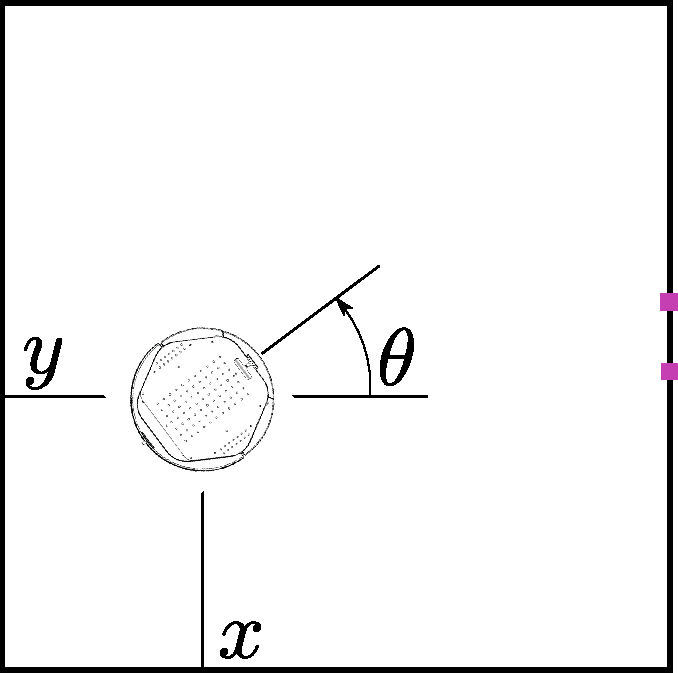
\includegraphics[width=.3\linewidth]{environment}
\caption{\label{fig:envir} Robot in its environment}
\end{figure}

\subsection{Expected work}

During the lab the files will be modified and others will be created.
At the end of the lab, please send by email a zip file allowing to compile and test the program.

You may answer the questions by inserting comments in the code at the corresponding lines.



\newpage

\section{Building the \texttt{Robot} class}

\subsection{Incomplete methods}


\begin{itemize}
\medskip\item[\textbf{\underline{Q1}}]  Compile and execute the program. According to the \texttt{main.cpp} file, the robot is following some velocity setpoints defined in the $(x,y,\theta)$ space. In which files are the following elements defined:
\begin{enumerate}
\item \texttt{DefaultEnvironment}
\item \texttt{DefaultCartesianSetpoint}
\item \texttt{Environment}
\end{enumerate}

\medskip\item[\textbf{\underline{Q2}}] Explain the signature of   \texttt{DefaultCartesianSetpoint}, especially the way to pass arguments. 
From the \texttt{main()} function, can \texttt{i} be modified in \texttt{DefaultCartesianSetpoint}? What about \texttt{vx}?

\medskip\item[\textbf{\underline{Q3}}] In practice it is often impossible to control a ground robot by sending $(x,y,\theta)$ velocities. A classical way to control such a robot is to send a setpoint with a linear velocity $v$ and an angular velocity $\omega$, expressed in the robot frame as shown in \Fig{fig:dd}.


\begin{figure}[h]\centering
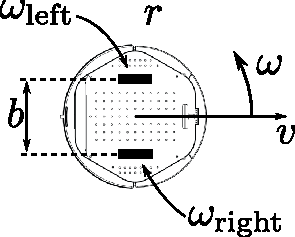
\includegraphics[width=.3\linewidth]{wheels}
\caption{\label{fig:dd} Differential drive model}
\end{figure}

The corresponding model is quite simple:
\begin{equation}
\left\{\begin{array}{ll}
\dot x &= v\cos \theta \\
\dot y &= v\sin \theta \\
\dot \theta &= \omega
\end{array}\right.
\end{equation}

Implement such a function in \texttt{Robot::MoveVW}. This method should compute the $(x,y,\theta)$ velocities from $(v,\omega)$ and then call the \texttt{Robot::MoveXYT} method. 

\medskip\item[\textbf{\underline{Q4}}] Now that a realistic way to control the robot is possible, should the \texttt{Robot::MoveXYT} method stay available for external use? What can we do in the \texttt{robot.h} file to make it impossible to use it from outside the \texttt{Robot} class?

\medskip\item[\textbf{\underline{Q5}}] When a robot is equipped with two actuated wheels, a simple model is the differential drive model, as shown in \Fig{fig:dd}. Assuming the two wheels have a radius $r$ and are separated with a distance $b$, then the kinematic model yields:
\begin{equation}\label{eq:dk}
\left\{\begin{array}{ll}
v &= \displaystyle r \frac{\omega_l + \omega_r}{2} \\
\omega &= \displaystyle r \frac{\omega_l - \omega_r}{2b}
\end{array}\right.
\end{equation}As in question 3, implement such a function in the \texttt{Robot::RotateWheels} method, so that it can be possible to control the robot by sending wheel velocities. You may want to define new attributes in the \texttt{Robot} class in order to initialize the radius and base distance through the \texttt{Robot::InitWheel} method. We use the following values:
\begin{equation}
\left\{\begin{array}{ll}
r &= 0.05 m \\
b &= 0.3 m
\end{array}\right.
\end{equation}
The method should rely on \texttt{Robot::MoveXYT} after having computed the $(x,y,\theta)$ velocities from $(\omega_l, \omega_r)$.

\medskip\item[\textbf{\underline{Q6}}] By using the \texttt{wheels\_init\_} attribute, make sure that it is impossible to do anything in \texttt{Robot::RotateWheels} if the radius and base have not been initialized.


\subsection{Velocity limits}

With the current simulation, we can control the robot:
\begin{itemize}
\item by sending linear and angular velocity setpoint with \texttt{Robot::MoveVW}
\item or by sending wheel velocities with \texttt{Robot::RotateWheels}
\end{itemize}

These two methods call \texttt{Robot::MoveXYT}\footnote{which should not be calable anymore from outside the \texttt{Robot} class} and the robot can reach any velocity. In practice, the wheels have a limited velocity at $\pm$80 round per minute (rpm).

\medskip\item[\textbf{\underline{Q1}}] Modify the \texttt{Robot::InitWheels} method in order to pass a new argument that defines the wheel angular velocity limit. You may need to define a new attribute of the \texttt{Robot} class to store this limit. Update the \texttt{main.cpp} file with the value in radian per second corresponding to 80 rpm.

\medskip\item[\textbf{\underline{Q2}}] Modify the \texttt{Robot::RotateWheels} method in order to ensure that the applied velocities $(\omega_l, \omega_r)$ are within the bounds.
The method should also print a message if the velocity setpoint is too high.
Note that if you just saturate the velocities, the robot motion will be different. A scaling is a better strategy, in this case we keep the same ratio between $\omega_l$ and $\omega_r$.

\medskip\item[\textbf{\underline{Q3}}] Although the robot actually moves by having its wheels rotate, it would be easier to be able to send linear and angular velocity setpoints. Modify the 
\texttt{Robot::MoveVW} method so that a $(v,\omega)$ setpoint is changed to a $(\omega_l,\omega_r)$ setpoint that will then be called through \texttt{Robot::RotateWheels}. Apply the default $(v,\omega)$ trajectory in the simulator. The inverse of model \eqref{eq:dk} yields:
\begin{equation}
\left\{\begin{array}{ll}
\omega_l &= \displaystyle \frac{v + b\omega}{r} \\
\omega_r &= \displaystyle \frac{v - b\omega}{r}
\end{array}\right.
\end{equation} 

\end{itemize}


\section{Sensors}

The \texttt{sensor.h} files defines a \texttt{Sensor} class that has four methods:
\begin{itemize}
\item \texttt{void Init}: initializes the relative pose between the sensor and the robot
\item \texttt{virtual void Update}: updates the measurement from the robot current position
\item \texttt{void Print}: prints the current measurement
\item \texttt{void Plot}: plots the measurement history       
\end{itemize}
The \texttt{Update} method is defined as a pure virtual function, which makes the \texttt{Sensor} class a abstract class. It is thus impossible to declare a variable to be of \texttt{Sensor} type, as this class is only designed to build daughter-classes depending on the sensor type.

The \texttt{Robot} class already has a attribute called \texttt{sensors\_} which is a vector of \texttt{Sensor*}. As the \texttt{Sensor} class is abtract it is forbidden to use it by itself, but pointers are still possible.


\subsection{Range sensors}


\begin{itemize}
\medskip\item[\textbf{\underline{Q1}}] Create a \texttt{sensor\_range.h} file that defines a \texttt{SensorRange} class that is derived from \texttt{Sensor}. The \texttt{Update} method has to be defined so that the code compiles. For now, just make the method print something to the screen.

\medskip\item[\textbf{\underline{Q2}}] Include this file in \texttt{main.cpp} and declare a \texttt{SensorRange} variable.  We will use a front range sensor placed at $(0.1, 0,0)$ in the robot frame. Call the \texttt{Update} method at the beginning of the \texttt{for} loop. Run the program and ensure that the sensor is updated.

\medskip\item[\textbf{\underline{Q3}}] In this question we will build the \texttt{Update} function. This sensor should return the distance to the first wall in its x-axis. The sensor can thus be simulated in two steps:
\begin{enumerate}
\item Compute the absolute position and orientation of the sensor. As the robot is passed to the \texttt{Update} method, we can use its own $(x_r,y_r,\theta_r)$ position and the relative position $(x_s,y_s,\theta_s)$ of the sensor to get the absolute sensor position:
\begin{equation}
\left\{\begin{array}{ll}
x &= x_r + x_s\cos\theta_r - y_s\sin\theta_r \\
y &= y_r + x_s\sin\theta_r + y_s\cos\theta_r \\
\theta &= \theta_r + \theta_s
\end{array}\right.
\end{equation}
\item Compute the distance to the nearest wall. In the environment variable, the walls are defined by a list of points available in \texttt{envir.walls}. \Fig{fig:dist} shows a configuration where the sensor is at $(x,y,\theta)$ and is facing a wall defined by $(x_1,y_1)$ and $(x_2,y_2)$.
\begin{figure}[h]\centering
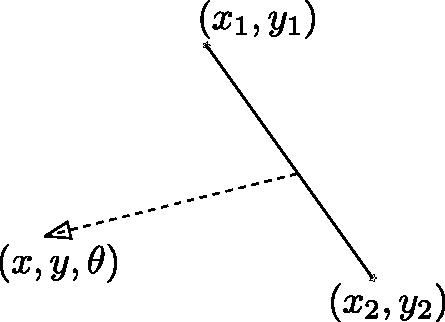
\includegraphics[width=.4\linewidth]{sensor}
\caption{Distance to a segment defined by two points.}
\label{fig:dist}
\end{figure}
In this case, the distance to the wall is:
\begin{equation}
d = \frac{x_{1} y_{2} - x_{1} y - x_{2} y_{1} + x_{2} y + x y_{1} - x y_{2}}{x_{1} \sin\theta - x_{2} \sin\theta - y_{1} \cos\theta + y_{2} \cos\theta}
\end{equation}
The computed distance is positive if the wall is in front of the sensor, and negative if it is behind (in this case this wall is actually not measured). Also, the denominator may be null if the wall is parallel to the sensor orientation.
\end{enumerate}
Define the \texttt{Update} function so that it updates the attribute \texttt{s} of the sensor with the distance to the nearest wall. 

\medskip\item[\textbf{\underline{Q4}}] At the end of the \texttt{Update} method, add the command to append the measurement history: \\\texttt{s\_history\_.push\_back(s\_);}\\
At the end of the program call the \texttt{Plot} method of the range sensor in order to display the measurements.
\end{itemize}
\end{document}
